%%%%%%%%%%%%%%%%%%%%%%%%%%%%%%%%%%%%%%%%
%% MCM/ICM LaTeX Template %%
%% 2021 MCM/ICM           %%
%%%%%%%%%%%%%%%%%%%%%%%%%%%%%%%%%%%%%%%%
\documentclass[12pt]{article}
\usepackage{geometry}
\geometry{left=1in,right=0.75in,top=1in,bottom=1in}

%%%%%%%%%%%%%%%%%%%%%%%%%%%%%%%%%%%%%%%%
% Replace ABCDEF in the next line with your chosen problem
% and replace 1111111 with your Team Control Number
\newcommand{\Problem}{A}
\newcommand{\Team}{2102677}
%%%%%%%%%%%%%%%%%%%%%%%%%%%%%%%%%%%%%%%%

\usepackage{newtxtext}
\usepackage{amsmath,amssymb,amsthm}
\usepackage{newtxmath} % must come after amsXXX

\usepackage{graphicx}
\usepackage{indentfirst}
%\usepackage{xcolor}
\usepackage{fancyhdr}
\lhead{Team \Team}
\rhead{}
\cfoot{}

\newtheorem{theorem}{Theorem}
\newtheorem{corollary}[theorem]{Corollary}
\newtheorem{lemma}[theorem]{Lemma}
\newtheorem{definition}{Definition}

%%%%%%%%%%%%%%%%%%%%%%%%%%%%%%%%
%================================
\usepackage{enumerate}%\item 需要
\usepackage{tabularx}% \table 
\usepackage{booktabs}% 	\toprule
\usepackage{float}%图片浮动
\usepackage{graphicx}
\usepackage{bm}% reference
\usepackage{indentfirst} 
\setlength{\parindent}{2em} %2em代表首行缩进两个字符
\usepackage{listings}%代码
%================================
%\usepackage{color}
\usepackage[table]{xcolor}
\usepackage{colortbl}
\definecolor{mygray}{gray}{.9}
\definecolor{mypink}{rgb}{.99,.91,.95}
\definecolor{mycyan}{cmyk}{.3,0,0,0}

%===========================================

\begin{document}
	\setcounter{page}{1} 
	
%\graphicspath{{.}}  % Place your graphic files in the same directory as your main document
%\DeclareGraphicsExtensions{.pdf, .jpg, .tif, .png}
\thispagestyle{empty}
\vspace*{-16ex}
\centerline{\begin{tabular}{*3{c}}
	\parbox[t]{0.3\linewidth}{\begin{center}\textbf{Problem Chosen}\\ \Large \textcolor{red}{\Problem}\end{center}}
	& \parbox[t]{0.3\linewidth}{\begin{center}\textbf{2021\\ MCM/ICM\\ Summary Sheet}\end{center}}
	& \parbox[t]{0.3\linewidth}{\begin{center}\textbf{Team Control Number}\\ \Large \textcolor{red}{\Team}\end{center}}	\\
	\hline
\end{tabular}}

%==========================================
\renewcommand{\abstractname}{Summary}

%=====================================
%%%%%%%%%%% Begin Summary %%%%%%%%%%%
% Enter your summary here replacing the (red) text
% Replace the text from here ...

\begin{center}
	\large\textbf{  { A System of Interstate Energy Cooperation Goals Based on Data Insight}}
	\end{center}
\begin{abstract}

In the terrestrial ecosystem, fungi are prominent agents since they act as the dominant decomposers in the carbon cycle and nutrient dynamic on the earth. Given that different species of fungi have different traits and life strategies, the decomposition rate varies vastly in a single flora family or a certain combination of them. Such difference provides a connection between the biological community and the ecosystem. Therefore, researches concentrating on the traits and interactions among different species of fungi are necessary in the process of the improvement of global biogeochemical model. Especially in today, studies have drawn much attention that globally the rate of release of $CO_{2}$ from the decomposition of microorganisms is similar to that of fossil-fuel combustion.

To address the challenge mentioned above, we proposed two basic models, one with focus on the decomposition process, the other on their interaction at the presence of multiple fungi species. With each of the two models is an extension model respectively. We also developed an algorithm using cellular automation process for co-ordination and validation of our models.

The first model, Single-species Decomposition Model (SDM), is established using the method of differential equations. A well-founded solution indicating the decomposition process is deduced with both qualitative and  quantitative analysis. Then we extend this model to Multi-species Decomposition Model (MDM) to further demonstrate the decomposition process.

The second model, Interactions between Multi-species Model (IMM) is built on the basis of Ulrich's method, more specifically, with Patch Matrices and Markov Process. Limited by its assumptions, the method is only appropriate for relatively slight environmental fluctuations. With our careful study and observation into the data sets, we propose a novel model, the Environmentally Conditioned Multi-species Model (ECMM) as an extension and possible attempt to refine this method, with more capability to have the environmental factors taken into consideration.

The algorithm, High-Precision Cellular-Automaton (HPCA), is a brand new method based on the traditional CA, but is both extended to have a really large scale to improve precision to fit in the continuous model, and uses a Flood Fill recursion to perform more effectively to get the visual graph. The cell algorithm is also based on Chebyshev Inequality and go through complete building process including Karnaugh map and Finite State Machine (FSM) analysis. HPCA is used widely for not only validating the two models we’ve built but also sensitivity test.

\textbf{Keywords}: Decomposition, Interaction, Environment, Cellular Automation.

\end{abstract}
% to here
%%%%%%%%%%% End Summary %%%%%%%%%%%

%%%%%%%%%%%%%%%%%%%%%%%%%%%%%%
\clearpage
\pagestyle{fancy}
% Uncomment the next line to generate a Table of Contents
\rhead{Page \thepage\ of 20}
\tableofcontents 
\newpage

%%%%%%%%%%%%%%%%%%%%%%%%%%%%%%


\section{Introduction}
\subsection{Problem Background}
Studies have shown that globally the rate of release of $CO_{2}$ from the decomposition of microorganisms (6 to 9.5Pg C/year [1,2]) is similar to that of fossil-fuel combustion (9.5Pg C/year in 2011 [3]). In the terrestrial ecosystem, fungi are prominent agents since they act as the dominant decomposers in the carbon cycle and nutrient dynamic on the earth. Their exclusive contributions include decomposition of organic and recalcitrant carbon, and transformations of nitrogen and phosphorus. 

Given that different species of fungi have different traits and life strategies, the decomposition rate varies vastly in a single flora family or a certain combination of fungi. This provides a connection between the biological community and the ecosystem. Therefore, researches concentrating on the traits and interaction among different species of fungi are necessary in the process of the improvement of global biogeochemical model.
\subsection{Restatement of the Problem}
\begin{itemize}
	\item Build a model with coexistence of multiple species of fungi in the decomposition process of ground litter and woody fibers.
	\item Expound interactions between different species of fungi including both short-term and long-term trends
	\item Predict possible advantage and disadvantage for each species and combinations with variation of  environmental patterns.
	\item Describe the importance and role of biodiversity on the decomposing system and variability of environment.
\end{itemize}
\subsection{Our work}

\begin{itemize}
	\item Establish a \textbf{Single-species Decomposition Model (SDM)} using method of Differential Equations (DEM). 
	\item Extend SDM to \textbf{Multi-species Decomposition Model} (MDM).
	\item Establish a \textbf{Model of Interactions between Multi-species} (IMM) using Patch Matrices Method (PMM) and Markov Process (MP), which performs competition between coexisting species based on probability distribution.
	\item Extend IMM to \textbf{Environmentally Conditioned Multi-species Model} (ECMM) to take environmental fluctuation into consideration.
	\item Establish a \textbf{High-precision Cellular Automation Algorithm} (HPCA) including essential data analysis. The algorithm is also used for validation of previous model.
\end{itemize}

A visualized working process is shown below.
\begin{figure}[H]%\usepackage{float}
	\small
	\centering
	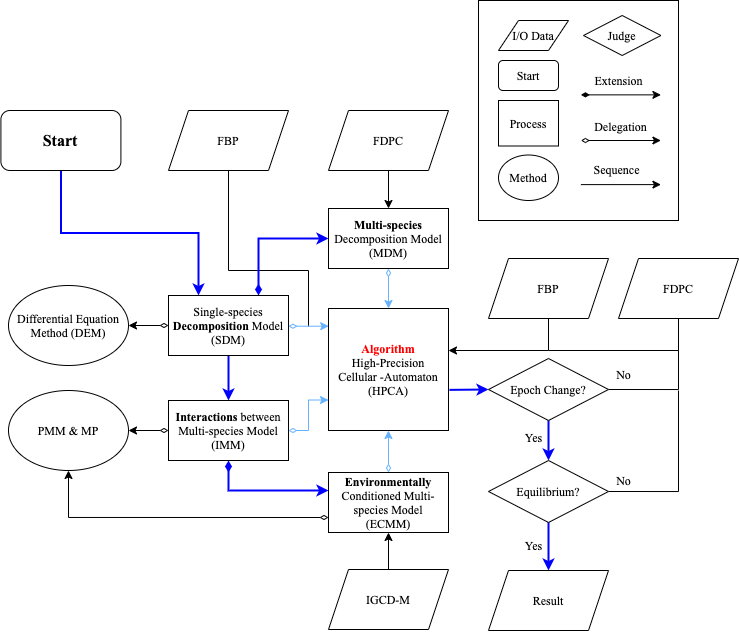
\includegraphics[width=15cm]{./pictures/workflow.png}
	\caption{Workflow of Our Modeling}\label{jj}
\end{figure}

%\newpage

\section{Preparation of the Models}

\subsection{Assumptions}
\begin{itemize}
	\item \textbf{Assumption 1: Part of the fungi in a colony dies if there is excess demand for nutrients.}
	
	In other words, birth and death in a colony happens simultaneously to keep the density at a balanced state when there are excess demand for nutrients.
	\item \textbf{Assumption 2: Interactions at the species level includes only competition.} 
	\item \textbf{Assumption 3: Difference between short- term and long-term interactions between fungal species is mainly reflected by environmental fluctuation.} 
	We consider environmental factors stay stable in the short term while oscillate with time in the long term.
\end{itemize}
\subsection{Notations}
All the symbols will be introduced once they are used.
\begin{table}[H]
	\begin{center}
		\caption{Notations}
		\begin{tabular}{cl}
			\toprule
			\multicolumn{1}{m{3cm}}{\centering Symbol}
			&\multicolumn{1}{m{8cm}}{\centering Definition}\\
			\midrule
			$M_{C}$&Competitive strength matrix\\
			$C$&Concentration of nutrients\\
			$C_{ext}$&Concentration of nutrients of external supply per unit time\\
			CBR&Crude birth rate per unit area\\
			CDR&Crude death rate per unit area\\
			$k_{1}$&Decomposition ability of single fungus\\
			$D$&Decomposition rate per unit area\\
			$P_{0}$&Demand for nutrients of single fungus\\
			$\rho$&Density of fungi\\
			$U$&Dominant eigenvector\\
			$k_{2}$&Growing ability of single fungus\\
			$T_{L}/T_{H}$&Lower/ higher boundary of temperature niche \\
			$M_{L}/M_{H}$&Lower/higher boundary of moisture niche\\
			NGR&Natural growth rate per unit area\\
			$T_{W}/M_{W}$&Niche width of temperature/ moisture\\
			$T_{O}/M_{O}$&Optimum temperature/ moisture\\
			$P$&Transition matrix\\
			$C_{i}$&Values related to the initial state\\
			
			\bottomrule
		\end{tabular}\label{Ntt}
	\end{center}
\end{table}
\section{Collection of Data}
Data utilized in our model takes two main roles, one acts as necessary information for the development of our model, the other is for validation. We cluster the collected data sets into three categories, including measurements of different species of fungi with their traits and environmental parameters considered, experimental outcomes of their interactions, and representative climate patterns as follows:
\begin{itemize}
	\item \textbf{Fungal Biogeography Performance (FBP):} includes growth and ecological performance traits of different species of fungi and climate-related data [4].
	\item \textbf{Fungal Diversity in Pairwise Competition  (FDPC):} includes outcomes of pairwise experiments comprising 37 species of fungi [6].
	\item \textbf{Fungal Interactions in Community (FIC):} includes results of the community consisting interactions among three species of fungi and respective individual microcosms [7].
	\item \textbf{Integrated Global Climate Data Monthly (IGCD-M):} includes integrate and homogenized global typical climate and atmosphere patterns [8].
\end{itemize}
\section{Model \uppercase\expandafter{\romannumeral1}: Short-term Single-species Decomposition Model}
In this model we consider a single-colony of short term under suitable environment. We develop the situation using differential equations and solve for a desirable equilibrium result using tools in MATLAB. Our assumptions and modeling process with results shown in graphs are shown below.
\subsection{Explanation of Parameters in the Model}
In this model suitable environment conditions are given, including suitable moisture and temperature for a single colony. Here we propose several parameters related to the traits of different kinds of fungi as follows:
\begin{itemize}
	\item \textbf{$P_{0}$:} a trait of a species, which is the major indicator which describes quantitatively the degree of "greed". In another word, $P_{0}$ represents the demand for nutrients of a single fungus. According to Assumption 1, we can obtain further cases as follows:
	\begin{equation}
		\begin{cases}
			excess\  supply,\  no\  fungal\  dies&if\  \frac{C}{\rho } \geqslant P_{0}\\ 
			excess\  demand,\  part\  of\  fungi\  die&if\  \frac{C}{\rho } <P_{0}
		\end{cases} 
	\end{equation} 
more detailed and quantitative information will be given in the construction of our model.
	\item $k_{1}$: a trait of a species, which indicates the decomposition ability of a single fungus. Note that this is different from the decomposition rate per area, D, as a whole. And the relation can be expressed as follows:
	\begin{equation}
		D=k_{1}\rho
	\end{equation} 
	This equation expresses that under given fungi density, a species with a stronger decomposition ability of a single fungus results in a higher rate of decomposition.
	\item $k_{2}$: a trait of a species, which indicates the growing ability of a fungus or the hyphal expansion rate. Equations describing the positive correlation between the crude birth rate (CBR) and $k_{2}$ is as follows (a stronger growing ability leads to a higher crude birth rate under given fungi density):
	\begin{equation}
		CBR=k_{2}\rho
	\end{equation}

\end{itemize}
\subsection{Model Construction Using Differential Equations}
We know that by definition, the natural growth rate (NGR) of a colony in a period of time equals to the difference between the crude birth rate (CBR) and the crude death rate (CDR):
\begin{equation}
	NGR=CBR-CDR
\end{equation}

NGR can also be defined as the rate of change of the density of the colony:
\begin{equation}
	NGR=\frac{\mathrm{d}\rho }{\mathrm{d}t} 
\end{equation}

Another relation lies below states that the difference between the nutrient concentration of external supply and decomposition rate equals the rate of change of the existing nutrient concentration:
\begin{equation}
	C_{ext}-D=\frac{\mathrm{d}C}{\mathrm{d}t} 
\end{equation}

From the Model Assumption we can obtain when there is excess demand: 	
\begin{equation}
	\begin{cases}
		CDR=0&if\  \frac{C}{\rho } \geqslant P_{0}\\ 
		CDR=\rho-\frac{C}{P_{0}}&if\  \frac{C}{\rho } <P_{0}
	\end{cases} 
\end{equation} 
where $\frac{C}{P_{0}}$ denotes the amount of fungi that is able to survive.
\subsection{Results and Analysis}
The results shows as a piecewise function:

\begin{equation}
	\begin{cases}
		\rho=C_{0}e^{k_{2}t}&if\  \frac{C}{\rho } \geqslant P_{0}\\ 
		\rho=C_{1}\frac{C_{ext}}{P_{0}(k_{1}+k_{2})}+C_{2}C_{ext}(k_{1}+k_{2})e^{-C_{3}\sqrt{k_{1}+k_{2}} t}\cos \left( \frac{k_{1}k_{2}}{P_{0}}t\right)+C_{4} &if\  \frac{C}{\rho } <P_{0}
	\end{cases} 
\end{equation} 
where $C_{i}$ is a set of values associated with the initial state. Justifications are as follows:

\begin{itemize}
	\item When there is excess supply, the density of fungi shows an exponential trend of increase. $C_{0}$ denotes the initial density of fungi.\\
	\item When there is excess demand, we try to cope with the solution of our model and some of the minor components in the solution are ignored. A fitted result is shown above. For further justification:
	\begin{enumerate}
		\item The density of fungi converges to a fixed value, $C_{1}\frac{C_{ext}}{P_{0}(k_{1}+k_{2})}$, which is positively correlated to $C_{ext}$, the external supply of nutrients and negatively correlated with $P_{0}$, the demand for nutrients of a single fungal. This is reasonable and conventional since more supply and less demand usual lead to higher density. Also, $\rho$ is negatively correlated with both $k_{1}$, the decomposition ability, and $k_{2}$, the growing ability. This is consistent with the findings described in a recent study [4].\\
		\item The second term in the equation, $C_{2}C_{ext}(k_{1}+k_{2})e^{-C_{3}\sqrt{k_{1}+k_{2}} t}\cos \left( \frac{k_{1}k_{2}}{P_{0}}t\right)$, represents the oscillation characteristic of the change of density with time. The frequency of the oscillation,  $\frac{k_{1}k_{2}}{P_{0}}$, indicates that with a stronger decomposing and growing ability, and less demand per fungus, the curve oscillates faster; the amplitude of the oscillation, $C_{ext}(k_{1}+k_{2})e^{-C_{3}\sqrt{k_{1}+k_{2}} t}$, decreases with time as the density of the colony tend to be more stable and adaptable to the environment through self-regulation. And the changes happens faster with time if the colony has a stronger ability of decomposition and growing, as denoted by the term $\sqrt{k_{1}+k_{2}}$. The magnitude of this amplitude is positively correlated with $C_{ext}$, $k_{1}$ and $k_{2}$ since with more nutrients supplied and stronger ability of decomposition and growing, the density changes more drastic.\\
		\item $C_{i}$ in the expression denotes some values associated with the initial state at $t=0$. For example, $C_{0}$ represents the initial density of the colony and $C_{3}$ may be related with the concentration of the nutrients and density of the colony initially.  
	\end{enumerate}
	\item The results are also visualized in the graph below:
\end{itemize}

\begin{figure}[H]%\usepackage{float}
	\small
	\centering
	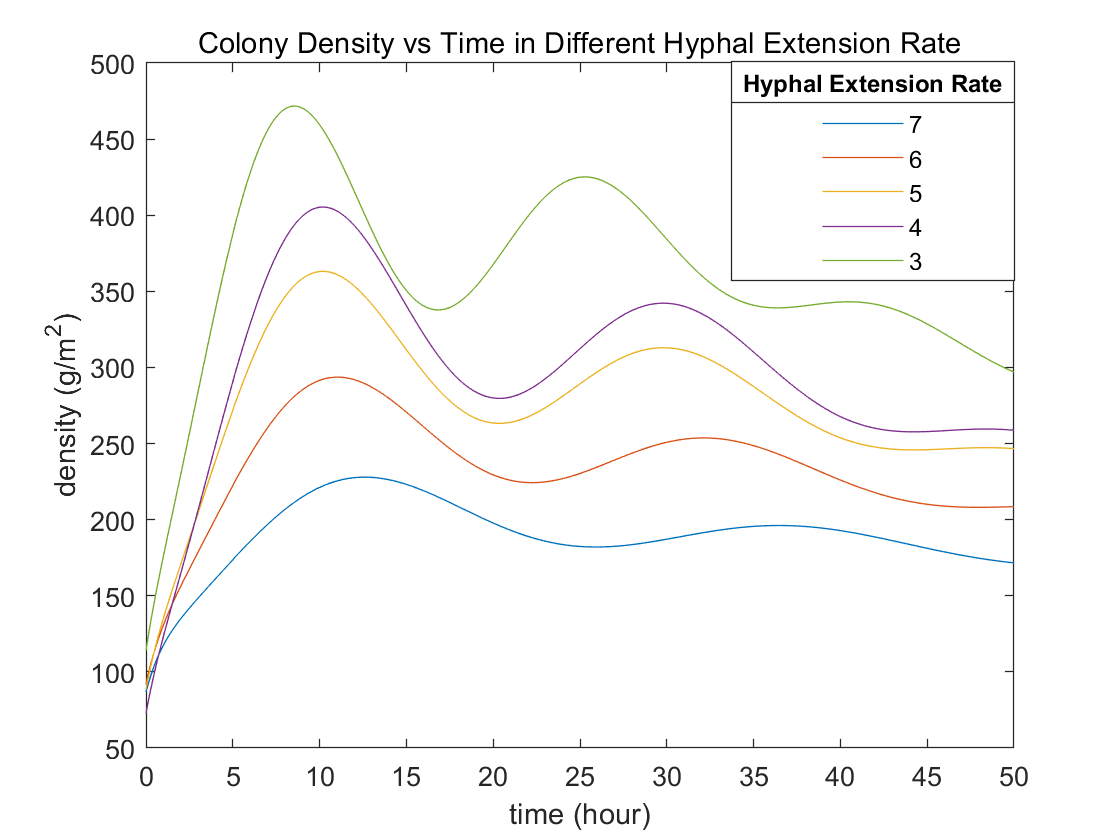
\includegraphics[width=14cm]{./pictures/model 1.png}
	\caption{Colony Density vs Time in Different Hyphal Extension Rate}\label{jj}
\end{figure}

\subsection{Extension: Short-term Multi-species Decomposition Model}
Separately, equations (1) $\sim$ (7) hold for all colonies of different species, which only vary in their traits and such difference can be embodied in parameters like $P_{0}$. Now we consider a situation at the presence of multiple species of fungi and look into their behavior in the decomposition process during the short term based on our single-colony model mentioned before. In this model we assume a relatively free living space for each of the different species. 

Given n species of fungi, we have new notations for the i-th strain as below:
\begin{table}[H]
	\centering
	\caption{Notations for Multi-strain Model}\label{y}
	\begin{tabularx}{0.9\textwidth}{cllll}
		\toprule
		
		Symbol & Definition\\
		\midrule
		
		\rowcolor{mygray}
		$C$&Concentration of nutrients\\
		\rowcolor{mygray}
		$C_{ext}$&Concentration of nutrients of external supply per unit time\\
		$CBR_{i}$&Crude birth rate per unit area of i-th strain\\
		$CDR_{i}$&Crude death rate per unit area of i-th strain\\
		$k_{1,i}$&Decomposition ability of single fungus of i-th strain\\
		$D_{i}$&Decomposition rate per unit area of i-th strain\\
		$P_{0,i}$&Demand for nutrients of single fungus of i-th strain\\
		$\rho_{i}$&Density of fungi of i-th strain\\
		$k_{2,i}$&Growing ability of single fungus of i-th strain\\
		$NGR_{i}$&Natural growth rate per unit area of i-th strain\\
		$C_{i,j}$&Values related to the initial state of i-th strain\\
		
		\bottomrule
	\end{tabularx}
\end{table}
where $C$ and $C_{ext}$ are environmental variables shared by all colonies. Accordingly, equation (6) becomes:
\begin{equation}
	C_{ext}-D_{i}=\frac{\mathrm{d}C}{\mathrm{d}t}
\end{equation}
as we consider several strains coexist in the same environment. Other equations changes in the same way.

In the multi-species decomposition model, each fungi has a different hyphal extension rate. The species with higher extension rate can grow faster. When the total density of the fungi colony reaches the critical point, some fungi will die because the lack of nutrition. In this model, we focus on the influence of hyphal extension rate to the species dominance. So after reaching the critical point, each species dies in a similar rate, but those who has a higher extension rate will grow faster and replace other species with a lower extension rate. In the multi-species decomposition model, without any change of environment variables, the species with higher hyphal extension rate will take the dominance because they recover faster than other species when the resource is limited.
\section{Model \uppercase\expandafter{\romannumeral2}:  Interactions between Multi-species Model}
Ulrich's method was originally a statistical framework using abundance matrices to estimate the contribution of intransitive competition in a community with patch matrices and Markov Process [5]. Limited by its assumptions, the method is only appropriate for relatively minor environmental fluctuations. On the basis of the database, we propose a possible way to find a link between the environmental variation and the network of competition among coexisting strains as an attempt to refine this method.
\subsection{Patch Matrices and Markov Process Analysis by Werner Ulrich}
\begin{itemize}
\item \textbf {The competition matrix ($M_{C}$):}In Ulrich's method, $M_{C}$ is derived from experiments. For m species, a matrix with size $m \times m$ is created in which every entry, $M_{C i,j}$ denotes the possibility that species i replaces species j in their interactions. 

Traditionally, the $M_{C}$ matrices are not column stochastic since all the diagonal elements are set to 1, meaning that the possibility that $M_{C i,i}$ replaces itself is 1. Thus it cannot be used in the Markov process. 
\item \textbf {The transition matrix ($P$):} Therefore we introduce the transition matrix $P$ in which every entry $P_{i,j}$ of the transition matrix $P$ is the probability of transition from species i to j and it is derived from $M_{C}$ using the equations below:
\begin{equation}
	\begin{aligned}
		P_{i,j}&=P\left( 1,\ldots ,m\right)  \left[ j\rightarrow i\right]\\
		&=\frac{1}{m-1} M_{C i,j}+\frac{1}{m-1} \sum^{m}_{k=1,k \neq i,j} M_{C j,k}P\left( 1,\ldots ,k-1,k+1,\ldots ,m\right)  \left[ j\rightarrow i\right]  
	\end{aligned}
\end{equation}
where $i \neq j$, that is, this equation gives the calculation for the non-diagonal elements in $P$ and for diagonal elements:
\begin{equation}
	P_{i,i}=\prod^{m}_{j=1,j \neq i} M_{C i,j}+\frac{1}{m-1} \sum^{m}_{k=1,k \neq i} M_{C i,k}P\left( 1,\ldots ,k-1,k+1,\ldots ,m\right)  \left[ i\rightarrow i\right]  
\end{equation}
\item \textbf{The dominant eigenvector ($U$):} $U$ is the respective dominant eigenvector that predicts the relative abundance distribution of different species at equilibrium. $U$ can be derived through Markov Process:

We know that for the transition probability, $P_{i,j}$, the limit exists:
\begin{equation}
	 \lim_{n\rightarrow \infty } P_{i,j}\left( n\right)  =\pi_{j} 
\end{equation}
or,
\begin{equation}
	P(n)=
	\begin{pmatrix}
		\pi_{1}&\pi_{2}  & \cdots  &\pi_{j} &\cdots \\ 
		\pi_{1}&\pi_{2}  & \cdots  &\pi_{j} &\cdots\\ 
		\vdots &\vdots  & \ddots & \vdots\\ 
		\pi_{1}&\pi_{2}  & \cdots  &\pi_{j} &\cdots\\
		\vdots &\vdots  &        &\vdots   &
	\end{pmatrix}
\end{equation}
then 
\begin{equation}
	U=(\pi_{1},\pi_{2},\hdots)
\end{equation}
as the limiting distribution or stationary distribution of the Markov Chain.
Specifically, $U_{i}$ denotes the probability of the $i_{th}$ species' dominance in the short term. 
\end{itemize}
\subsection{Calculation Results and Analysis with 4 Examples}
Here are four examples, each with three species of fungi, as illustration of our model. In each case, $M_{C}$ is derived from our main database. $P$ is calculated using equations (10) and (11) and $U$ is from equations (12) and (14).

These four experiments together reveal the difference in the prediction of species richness and probability distribution between perfectly transitive competition (Example 1) and  non-transitive competition (Example 2 to 4) environment. And the more even in the comparison of their initial strengths (in the competition matrix), the more even outcome will be derived. Just as the rock-scissors-paper game, intransitive competitive network generates loops of competitive strength [9].
\begin{table}[H]
	\centering
	\begin{minipage}[H]{0.35\textwidth}
	\centering
	\setlength{\tabcolsep}{3mm}{
	\begin{tabular}{|l|l|l|l|l}
		\cline{1-4}
		$M_{C1}$& A & B & C \\ \cline{1-4}
		A & 1.00 & 1.00 & 1.00 \\ \cline{1-4}
		B & 0.00 & 1.00 & 1.00 \\ \cline{1-4}
		C & 0.00 & 0.00 & 1.00 \\ \cline{1-4}
	\end{tabular}}
	\end{minipage}
\begin{minipage}[H]{0.2\textwidth}
	\centering
	\setlength{\tabcolsep}{3mm}{
	\begin{tabular}{|l|l|l|l|l}
		\cline{1-4}
		$P_{1}$& A & B & C \\ \cline{1-4}
		A & 1.00 & 1.00 & 0.50 \\ \cline{1-4}
		B & 0.00 & 0.00 & 0.50 \\ \cline{1-4}
		C & 0.00 & 0.00 & 0.00 \\ \cline{1-4}
	\end{tabular}}
\end{minipage}
	\begin{minipage}[H]{0.4\textwidth}
	\centering
	\setlength{\tabcolsep}{3mm}{	
	\begin{tabular}{|l|l|}
		\hline
		A & 1.00 \\ \hline
		B & 0.00 \\ \hline
		C & 0.00 \\ \hline
	\end{tabular}}
	\end{minipage}
\caption{Example 1: From $M_{C1}$ to $P_{1}$ to $U_{1}$}
\end{table} 
 
 
\begin{table}[H]
	\centering
	\begin{minipage}[H]{0.35\textwidth}
		\centering
		\setlength{\tabcolsep}{3mm}{
			\begin{tabular}{|l|l|l|l|l}
				\cline{1-4}
				$M_{C2}$& A & B & C \\ \cline{1-4}
				A & 1.00 & 0.60 & 0.60 \\ \cline{1-4}
				B & 0.40 & 1.00 & 0.60 \\ \cline{1-4}
				C & 0.40 & 0.40 & 1.00 \\ \cline{1-4}
		\end{tabular}}
	\end{minipage}
	\begin{minipage}[H]{0.2\textwidth}
		\centering
		\setlength{\tabcolsep}{3mm}{
			\begin{tabular}{|l|l|l|l|l}
				\cline{1-4}
				$P_{2}$& A & B & C \\ \cline{1-4}
				A & 0.36 & 0.48 & 0.42 \\ \cline{1-4}
				B & 0.32 & 0.24 & 0.42 \\ \cline{1-4}
				C & 0.32 & 0.28 & 0.16 \\ \cline{1-4}
		\end{tabular}}
	\end{minipage}
	\begin{minipage}[H]{0.4\textwidth}
		\centering
		\setlength{\tabcolsep}{3mm}{	
			\begin{tabular}{|l|l|}
				\hline
				A & 0.41 \\ \hline
				B & 0.32 \\ \hline
				C & 0.27 \\ \hline
		\end{tabular}}
	\end{minipage}
	\caption{Example 2: From $M_{C2}$ to $P_{2}$ to $U_{2}$}
\end{table} 


\begin{table}[H]
	\centering
	\begin{minipage}[H]{0.35\textwidth}
		\centering
		\setlength{\tabcolsep}{3mm}{
			\begin{tabular}{|l|l|l|l|l}
				\cline{1-4}
				$M_{C3}$& A & B & C \\ \cline{1-4}
				A & 1.00 & 0.20 & 0.20 \\ \cline{1-4}
				B & 0.80 & 1.00 & 0.80 \\ \cline{1-4}
				C & 0.80 & 0.20 & 1.00 \\ \cline{1-4}
		\end{tabular}}
	\end{minipage}
	\begin{minipage}[H]{0.2\textwidth}
		\centering
		\setlength{\tabcolsep}{3mm}{
			\begin{tabular}{|l|l|l|l|l}
				\cline{1-4}
				$P_{3}$& A & B & C \\ \cline{1-4}
				A & 0.40 & 0.18 & 0.12 \\ \cline{1-4}
				B & 0.48 & 0.64 & 0.72 \\ \cline{1-4}
				C & 0.48 & 0.18 & 0.16 \\ \cline{1-4}
		\end{tabular}}
	\end{minipage}
	\begin{minipage}[H]{0.4\textwidth}
		\centering
		\setlength{\tabcolsep}{3mm}{	
			\begin{tabular}{|l|l|}
				\hline
				A & 0.15 \\ \hline
				B & 0.63 \\ \hline
				C & 0.22 \\ \hline
		\end{tabular}}
	\end{minipage}
	\caption{Example 3: From $M_{C}$ to $P_{3}$ to $U_{3}$}
\end{table} 


\begin{table}[H]
	\centering
	\begin{minipage}[H]{0.35\textwidth}
		\centering
		\setlength{\tabcolsep}{3mm}{
			\begin{tabular}{|l|l|l|l|l}
				\cline{1-4}
				$M_{C4}$& A & B & C \\ \cline{1-4}
				A & 1.00 & 0.20 & 0.70 \\ \cline{1-4}
				B & 0.80 & 1.00 & 0.70 \\ \cline{1-4}
				C & 0.30 & 0.30 & 1.00 \\ \cline{1-4}
		\end{tabular}}
	\end{minipage}
	\begin{minipage}[H]{0.2\textwidth}
		\centering
		\setlength{\tabcolsep}{3mm}{
			\begin{tabular}{|l|l|l|l|l}
				\cline{1-4}
				$P_{4}$& A & B & C \\ \cline{1-4}
				A & 0.14 & 0.17 & 0.46 \\ \cline{1-4}
				B & 0.68 & 0.56 & 0.46 \\ \cline{1-4}
				C & 0.18 & 0.27 & 0.09 \\ \cline{1-4}
		\end{tabular}}
	\end{minipage}
	\begin{minipage}[H]{0.4\textwidth}
		\centering
		\setlength{\tabcolsep}{3mm}{	
			\begin{tabular}{|l|l|}
				\hline
				A & 0.22 \\ \hline
				B & 0.57 \\ \hline
				C & 0.21 \\ \hline
		\end{tabular}}
	\end{minipage}
	\caption{Example 4: From $M_{C4}$ to $P_{4}$ to $U_{4}$}
\end{table}  

\subsection{Extension: Environmentally Conditioned Multi-species Model}
As mentioned previously, the limit matrix, $U$, derived from Ulrich's method could not bear slightly drastic environmental fluctuations since such outcome can be overridden by environmental heterogeneity [5]. By careful study, we now propose a possible way based on Markov Process to refine this method, taking environmental changes into consideration. This is also a model of multi-species in the long term.

First we define coefficients of the influence of temperature and moisture for species i:
\begin{equation}
	\begin{aligned}
	T_{i}(t)&=f(T(t), T_{L,i}, T_{H,i}, T_{W,i}, T_{O,i})\\
	&=p_{1}((T_{W})^2-(T(t)-T_{O})^2+p_{2})(p_{3}-T_{W})
	\end{aligned}
\end{equation}
\begin{equation}
	\begin{aligned}
	M_{i}(t)&=g(M(t), M_{L,i}, M_{H,i}, M_{W,i}, M_{O,i})\\
	&=q_{1}((M_{W})^2-(M(t)-M_{O})^2+q_{2})(q_{3}-M_{W})
	\end{aligned}
\end{equation}

\begin{figure}[H]
	\small
	\centering
	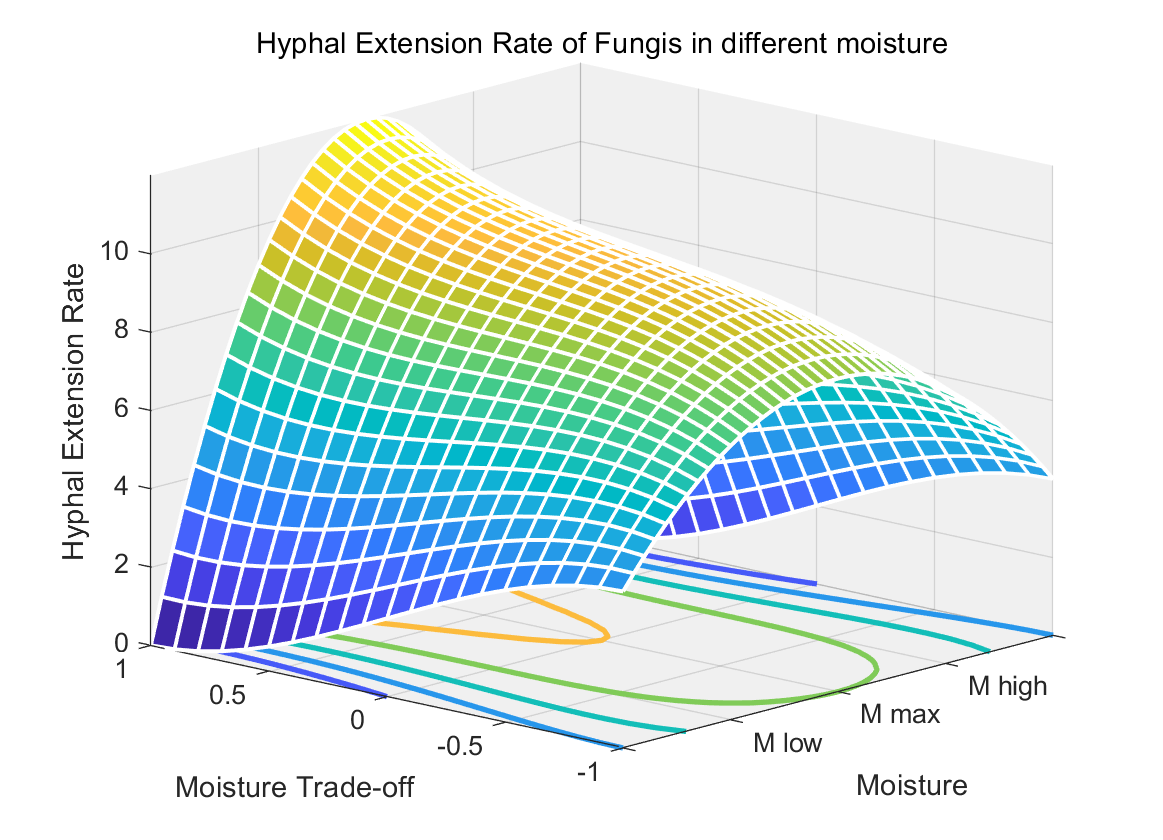
\includegraphics[width=15cm]{./pictures/env.png}
	\caption{HER vs Moisture}\label{jj}
\end{figure}
Based on our careful observation and evaluation to documents and data sets, we generate a fit surface for the moisture trade-off and environment moisture. The general trend is that the species with more tolerance is more stable but has a lower max hyphal extension rate, while the species with more dominance has a higher max extension rate but is less stable. Through previous research, we find that the species with higher hyphal extension rate will take the dominance. So when the experiment condition is suitable for the growth of fungi, the species with more dominance will take the dominance, and when the experiment condition is not suitable, the species with more tolerance will take the dominance.

Then at time t, the competition matrix, $C$:
\begin{equation}
	C_{i,j}(t)=h(T_{i}(t), M_{i}(t), T_{j}(t), M_{j}(t), \Delta t)
\end{equation}
where $\Delta t$ is regarded as the step length or the time interval of Markov Process and is related to the growth rate of Fungi. 

Now we can derive $P_{i,j}(t)$ from equation (10) and (11) by replacing $M_{C i,j}$, which is time-independent with our new matrix $C_{i,j}(t)$. To realize it numerically, we can write the Markov Chain as follows: 

\begin{equation}
	U_{i}(t+\Delta t)=\sum^{m}_{j=1} P_{i,j}(t)U_{i}(t)
\end{equation}
then the probability matrix can be derived as:
\begin{equation}
	\begin{pmatrix}
		p_{1,1}&p_{1,2}  & \cdots  &p_{1,n}  \\ 
		p_{2,1}&p_{2,2}  & \cdots  &p_{2,n} \\ 
		\vdots &\vdots  & \ddots\\ 
		p_{n,1}&p_{n,2}  & \cdots  &p_{n,n} \\
	\end{pmatrix}
\end{equation}

The final step is to compute the Poincare Map, $U_{t+k\Delta t}$, from one time point to any next time point:
\begin{equation}
	U(t+k\Delta t)=(\prod^{k}_{i=0}P(t+i\Delta t))U(t)
\end{equation}

Through the analysis to the relationship between environment variables and trade-offs, we can find that at different environment conditions, there exists a fungi with the highest hyphal extension rate. When the species diversity is high enough, an intransitive competition is much more possible, so the dominance probability is more balanced and various species may live together. 

Compared to single species, at different environment conditions, there will be one species takes the dominance among multi-species, which has the highest hyphal extension rate and decomposition rate. That dominant species must have a decomposition rate no lower than the single species. so with an interval of environment variables, the dominant decomposition rate is higher than the single species. So the species diversity promotes to the decomposition rate of fungi colony.


\section{Algorithm Realization Using Cellular Automation}
\begin{figure}[H]
	\small
	\centering
	\includegraphics[width=17cm]{./pictures/algorithm.png}
	\caption{The Structure of the Cellular Automation Algorithm}\label{jj}
\end{figure}
\subsection{Overview of the Algorithm}
\begin{itemize}
	\item \textbf{Indirect Parameters:} parameters indirectly related to our algorithm (HPCA) and relatively closer to the logic – the Temperature (T), Moisture (M), the Moisture Trade-off (MT) and the Hyphal Extension Rate (HER) of a certain species. 
	\item \textbf{WRM:} a function in C++ called Weight Resize Macro (WRM) to process the indirect variables based on data analysis.
	\item \textbf{Direct Parameters:} After the pre-processing of the raw (indirect) parameters, we now gain the 4 direct parameters - Soil Distribution ($d_S$), Colony Distribution ($d_C$), Recomposition Rate ($v_R$) and Decomposition Rate ($v_D$). These parameters are designed for our main algorithm (HPCA) after the Parameter Selection Macro(PSM).
	\item \textbf{PSM:} the function which takes the user input Process Selection Signal (sig) to choose the  parameter in the process (1 out of 4) the user wants. 
	\item \textbf{Principal Process:} 4 processes, including SSDP (Short-term Single-cell Decomposition Process, 00), LSDP (Long-term Single-cell Decomposition Process, 01), SMDP (Short-term Multiple-cell Decomposition Process, 10), and LMDP (Long-term Multiple-cell Decomposition Process, 11). After the user sets the Process Selection Signal (sig), the starter x index (i) and the starter y index (j), it completes the Cellular Automaton algorithm using conditioned recursion, principally, Flood Fill. 
	
	\end{itemize}

\subsection{Data processing and Analysis for WRM}
To quantify the relation between the indirect and direct parameters for WRM, it is essential for us to form a reasonable observation from previous data.
Here are two graphs we derived using MATLAB utilizing data set FBP which demonstrate the relation between density, moisture and temperature respectively. 
\begin{figure}[!htbp]
	\small
	\centering
	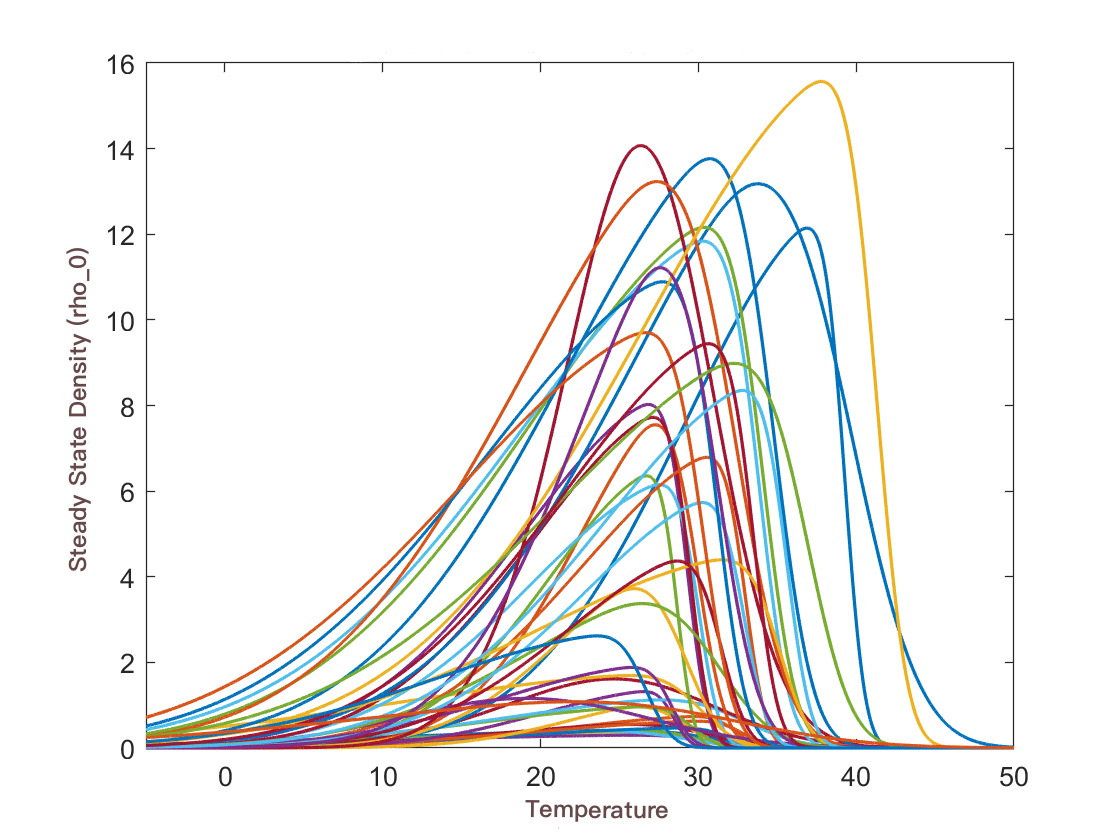
\includegraphics[width=8cm]{./pictures/temp.png}
	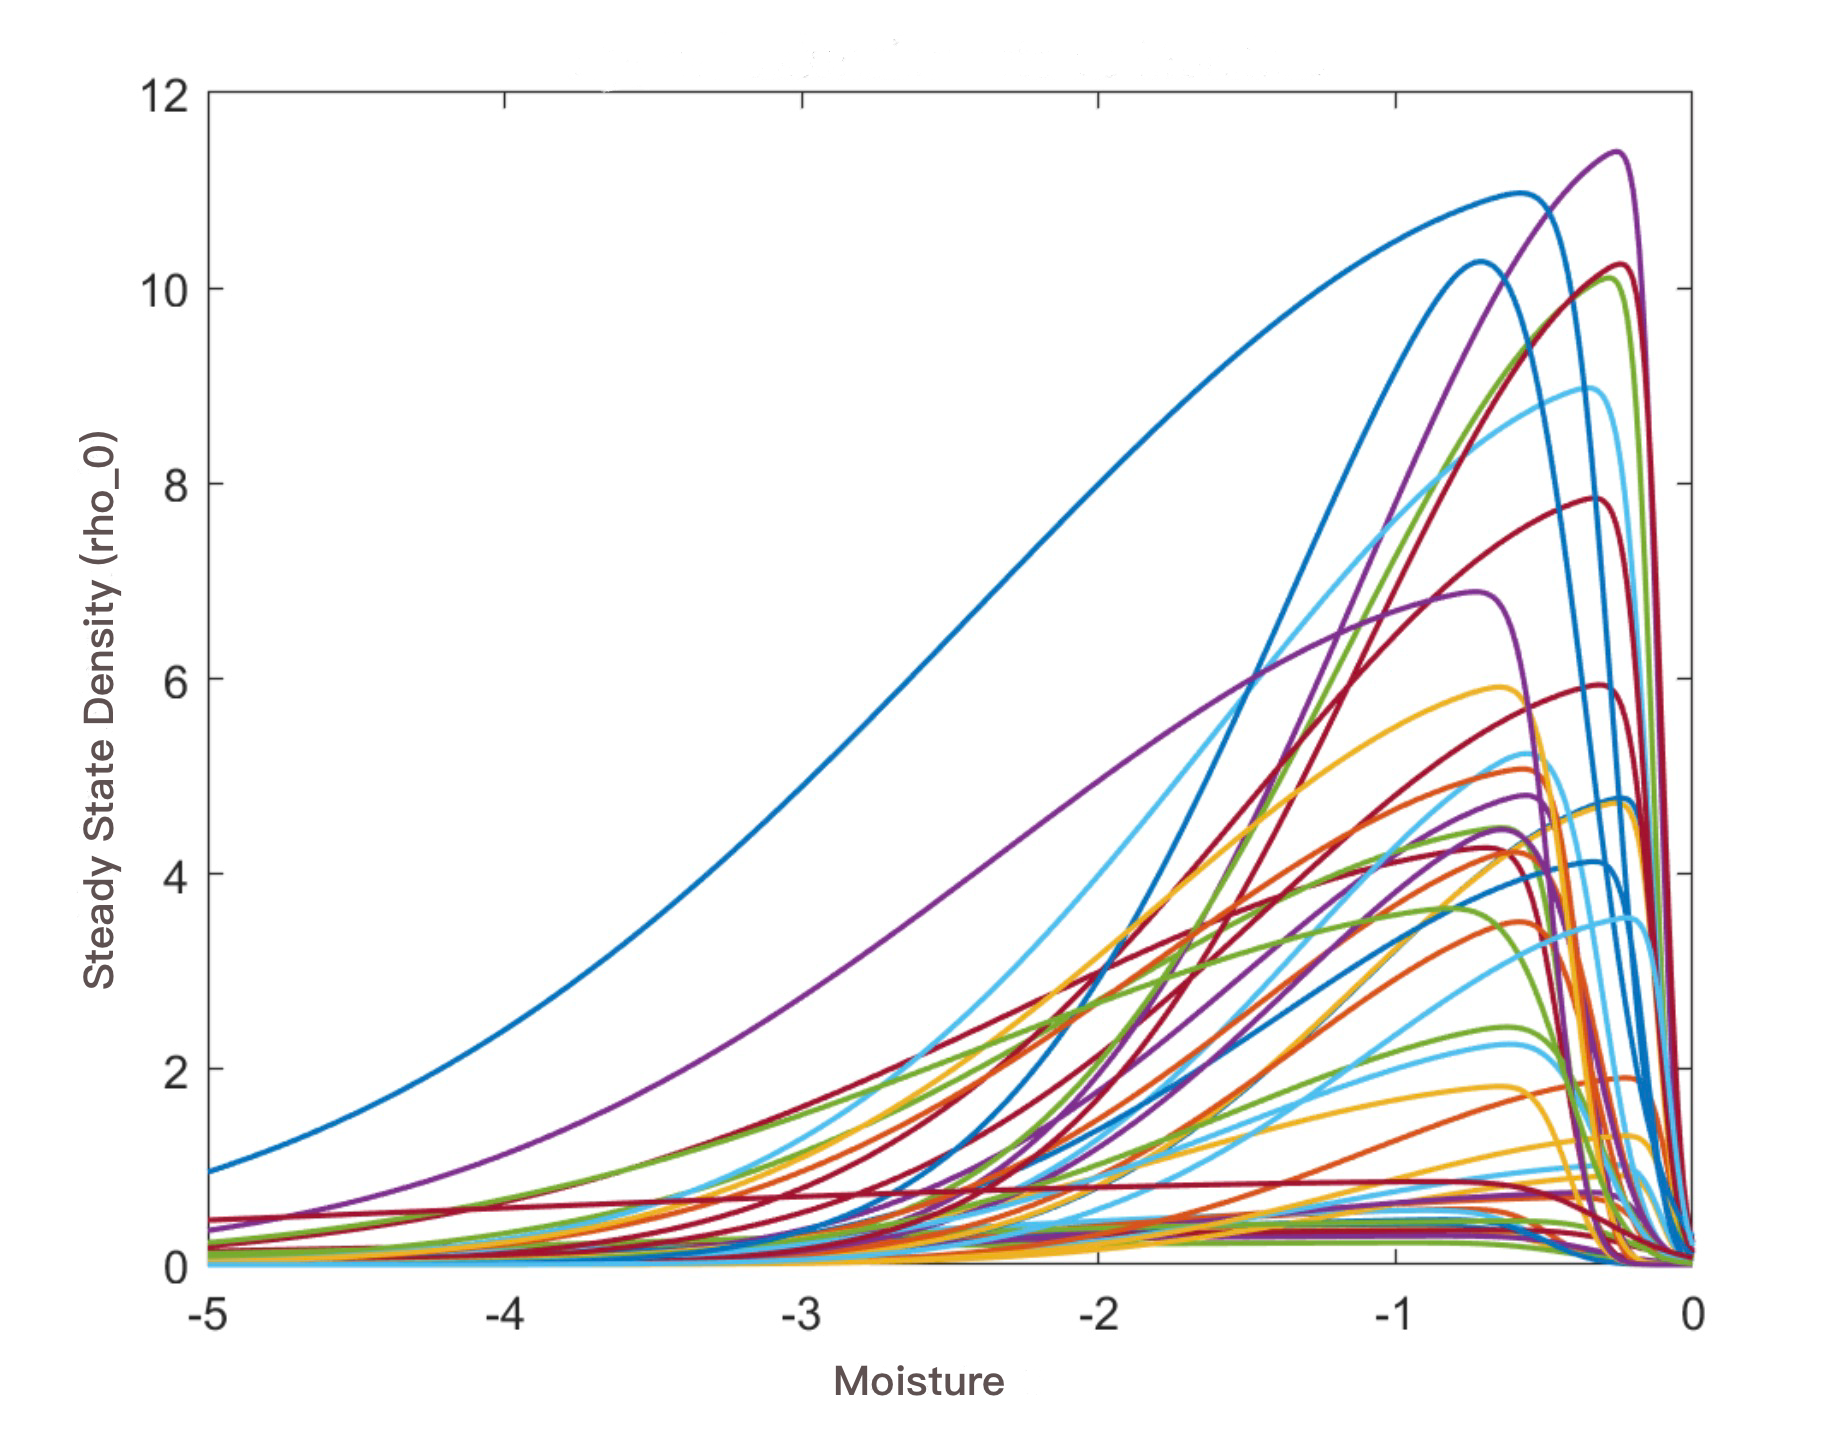
\includegraphics[width=7.5cm]{./pictures/moisture.png}
	\caption{Density vs Temperature (left) and Density vs Moisture (right)}\label{nt}
\end{figure}

Then we fit the curve using regression analysis. The responding outcomes from the Statistic Package for Social Science (SPSS) are shown below:

\begin{figure}[!htbp]
	\small
	\centering
	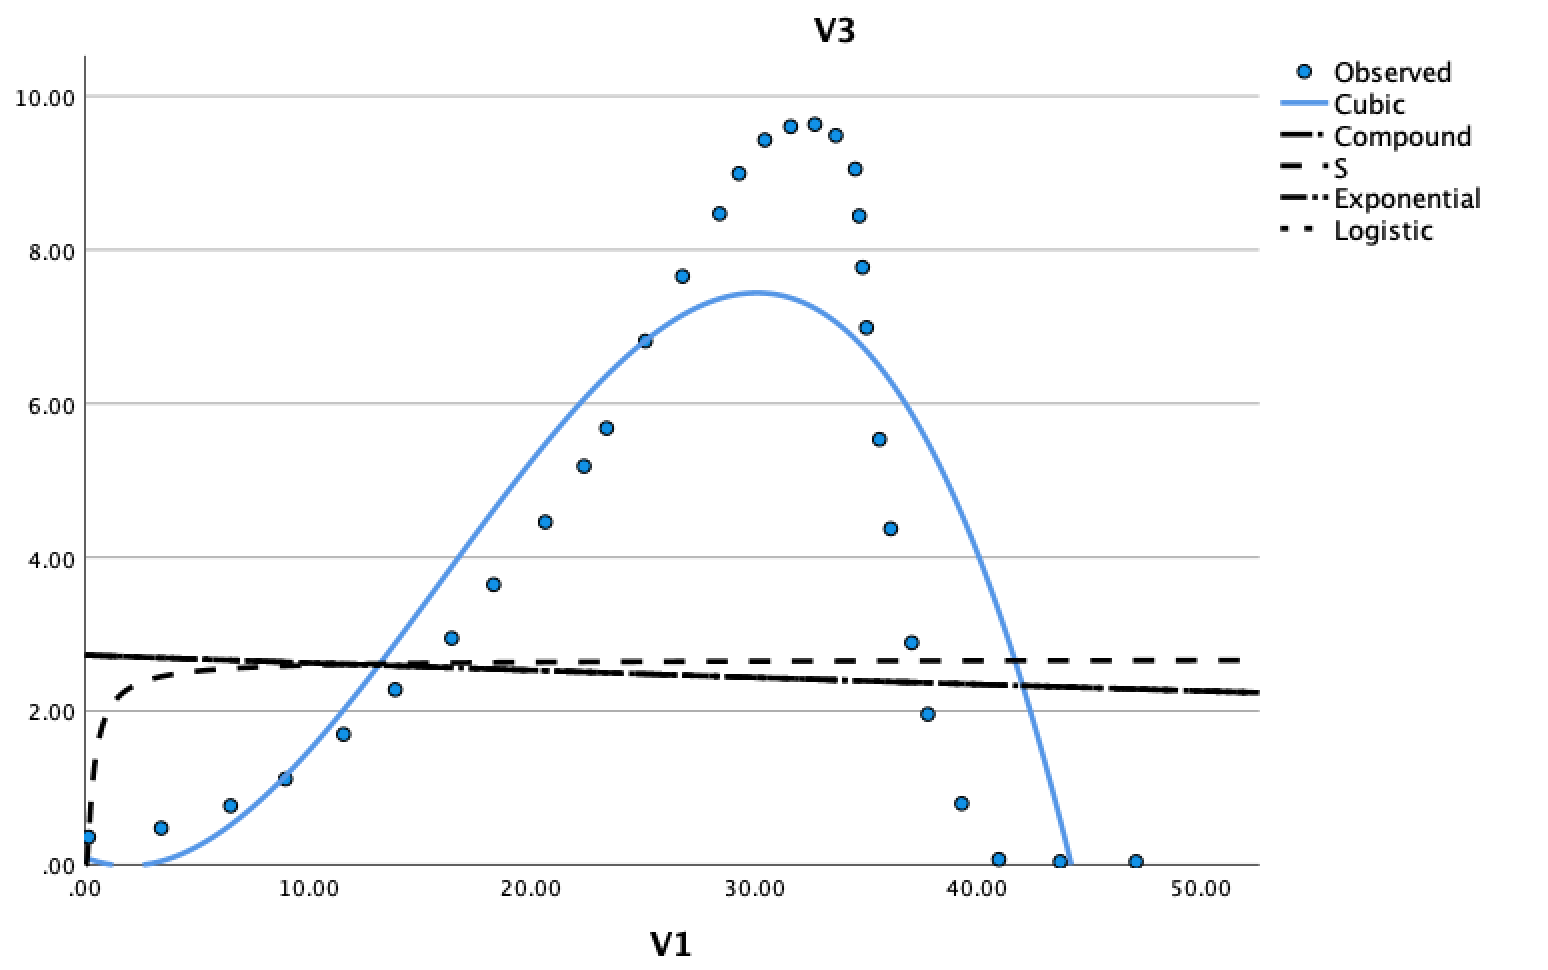
\includegraphics[width=8cm]{./pictures/temp1.png}
	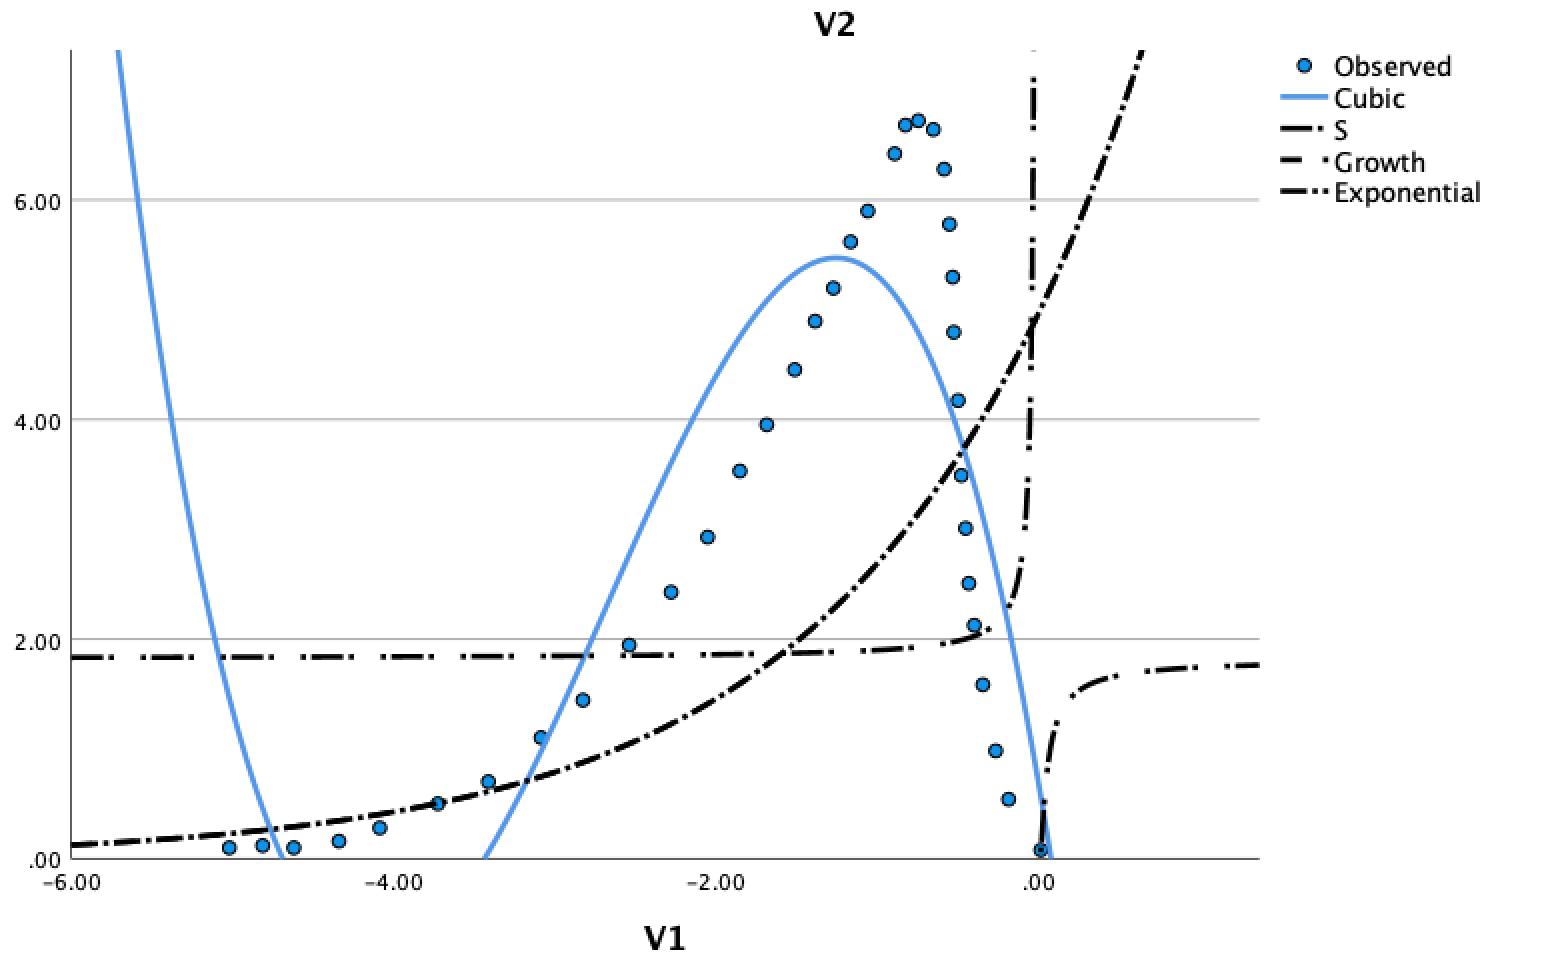
\includegraphics[width=8.5cm]{./pictures/moisture1.png}
	\caption{Density vs Temperature (left) and Density vs Moisture (right)}\label{nt}
\end{figure}
The light blue solid line in each graph represents a successful fit. The detailed equations are as follows:
\begin{equation}
	\rho (T)=-0.000664T^3-0.0319T^2-0.114T+0.0942
\end{equation}

\begin{equation}
	\rho (M)=-0.548M^3-4.41M^2-8.49M+0.679
\end{equation}

To further convince the credibility of our computation, we compared our results with statistics from other data set in both qualitative and quantitative justifications. Similar process is applied to evaluate other relations. 

In addition to the equations, conventions of default values are also given as follows based on data set FBP:
\begin{table}[H]
	\caption{Default Values for the Parameters}
	\label{tab:my-table}
	\centering
	\begin{tabular}{llll}
		\hline
		Input Parameter & Default Value & Output Parameter & Default Value \\ \hline
		Temperature (T) & 22 ℃  & Soil Distribution ($d_S$)  &  Normal Distribution             \\
		Moisture (M)  & -0.5 MPa & Colony Distribution ($d_C$) &  Single Parent Colony \\
		Moisture Trade-off (MT)& 2.08 & Soil Recomposition Rate($v_R$)  & 0   \\
		Hyphal Extension Rate (HER)& 4.82 mm/day & Soil Decompotition Rate($v_D$) & 0.8 (mm/s in HPCA)\\ 
		\cline{1-4}
	\end{tabular}
\end{table}

\subsection{Illustration of the Logic}
\begin{table}[H]
	\caption{Basic Information of the Algorithm}
	\label{tab:my-table}
	\centering
	\begin{tabular}{ll}
		\hline
		Model & HPCA, High-precision Cellular Automation \\ \hline
		Algorithm   & Flood Fill, Recursion         \\
		Language    & C++             \\
		States      & Initial, Occupied, Done              \\
		Graph Simul.& Matrix   \\
		Ideology    & Local Feature Theorem    \\
	    \cline{1-2}
	\end{tabular}
\end{table}

\begin{figure}[H]
	\small
	\centering
	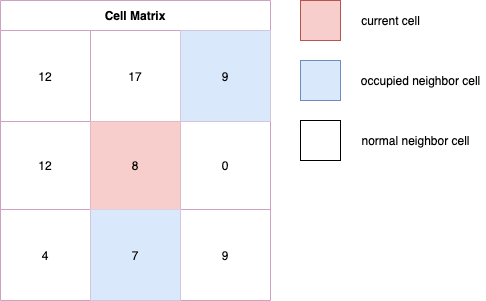
\includegraphics[width=12cm]{./pictures/cell illustration.png}
	\caption{Cell Matrix Illustration}\label{jj}
\end{figure}

The number in each grid means the remaining mass of nutrients per area (MPA) inside this grid. The red-colored grid represents the current cell while the blue-colored grid means that this grid is occupied now. Then we derive the K-Map as shown below:

\begin{figure}[h]
	\small
	\centering
	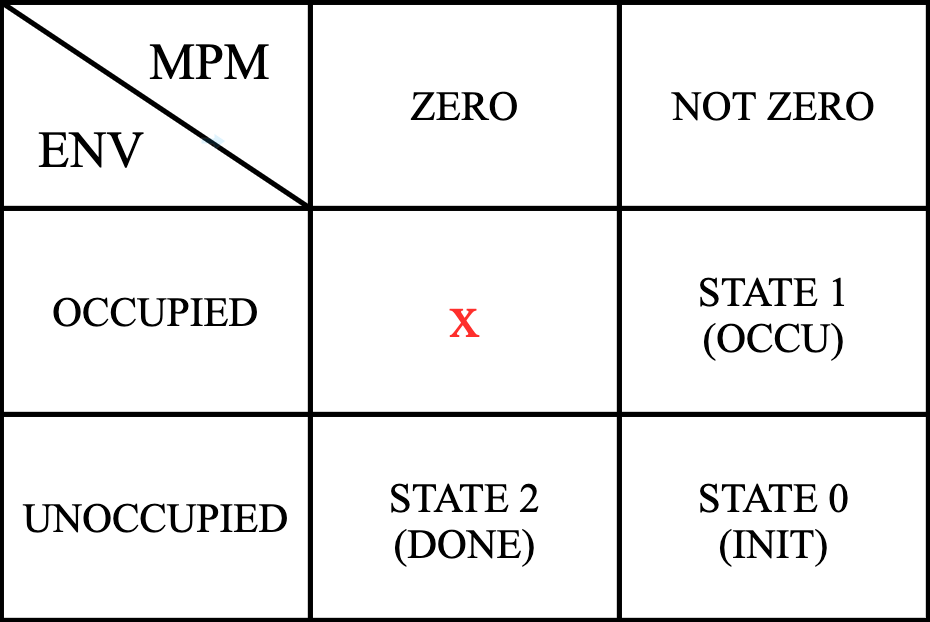
\includegraphics[width=7cm]{./pictures/K-Map.png}
	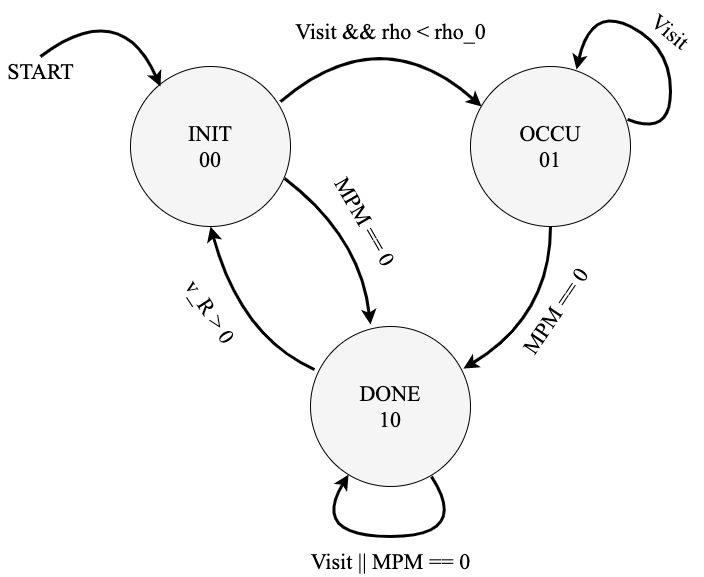
\includegraphics[width=8cm]{./pictures/FSM.png}
	\caption{Illustration of K-Map (left) and Finit State Machine (right)}\label{nt}
\end{figure}

According to the K-Map, we design the Finite State Machine (FSM) as shown in the Figure above on the right.
\begin{itemize}
\item (Outer) Goto INIT state when receiving signal START.
\item (INIT) Goto OCCU state when this cell is visited and the current density < the edge-case density. Goto DONE state when Mass Per square Meter (MPM) is 0.
\item (OCCU) Goto DONE state when MPM becomes 0. Stay if visited twice.
\item (DONE) Goto INIT state when Recomposition Rate ($v_{R}$) $>0$. Stay if visited again or MPM is zero.
Note. When in OCCU state, it’s forbidden to goto INIT state.
\end{itemize}
 
\subsection{Visualized Results}
The HPCA outputs a graph after each epoch and can be taken as working continuously. Also, as HPCA applies n from small to pretty large (up to n = 1,500), this Cellular Automaton is called High-Precision Cellular-Automaton, which covers the shortcoming that CA is usually taken as a discrete model so that it’s not so applicable to a continuous problem. Here are the results produced by our algorithm with different parameters:

\begin{figure}[!htbp]
	\small
	\centering
	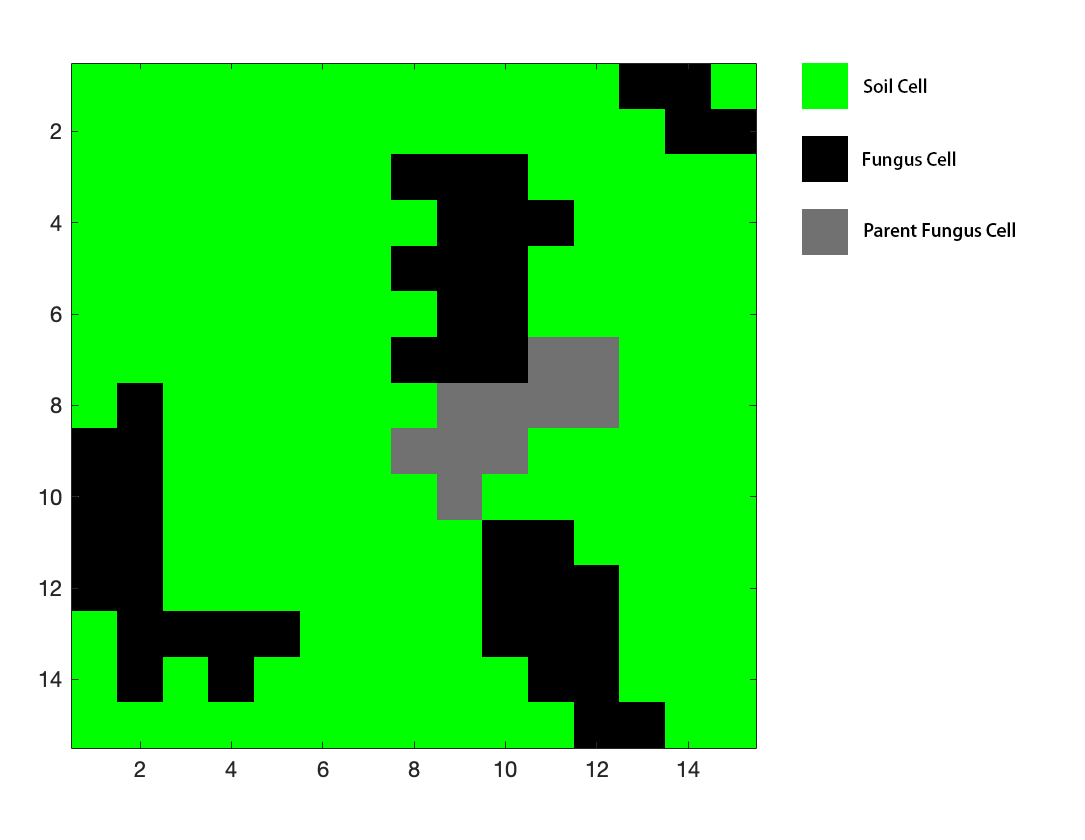
\includegraphics[width=8cm]{./pictures/cell1.png}
	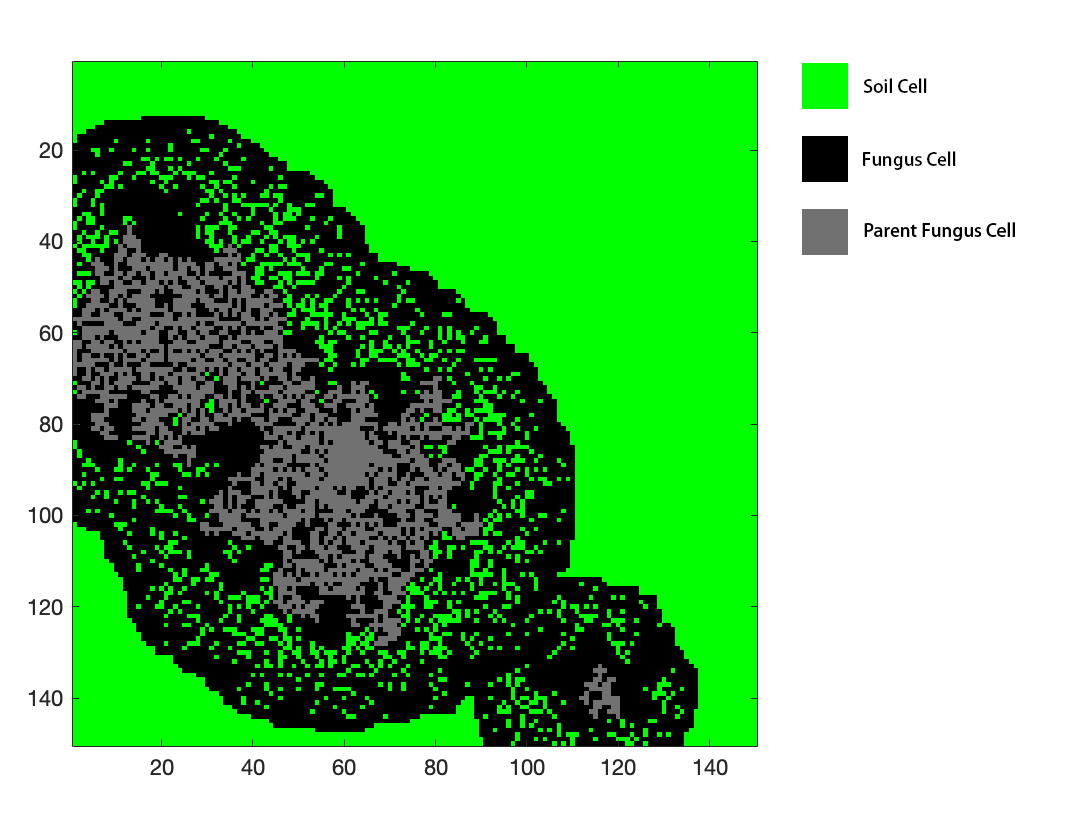
\includegraphics[width=8cm]{./pictures/cell2.png}
	\caption{SSDP at equilibrium, n=15, Parent=1 (left) and SSDP at equilibrium, n=150, Parent=3 (right)}\label{nt}
\end{figure}

\begin{figure}[H]
	\small
	\centering
	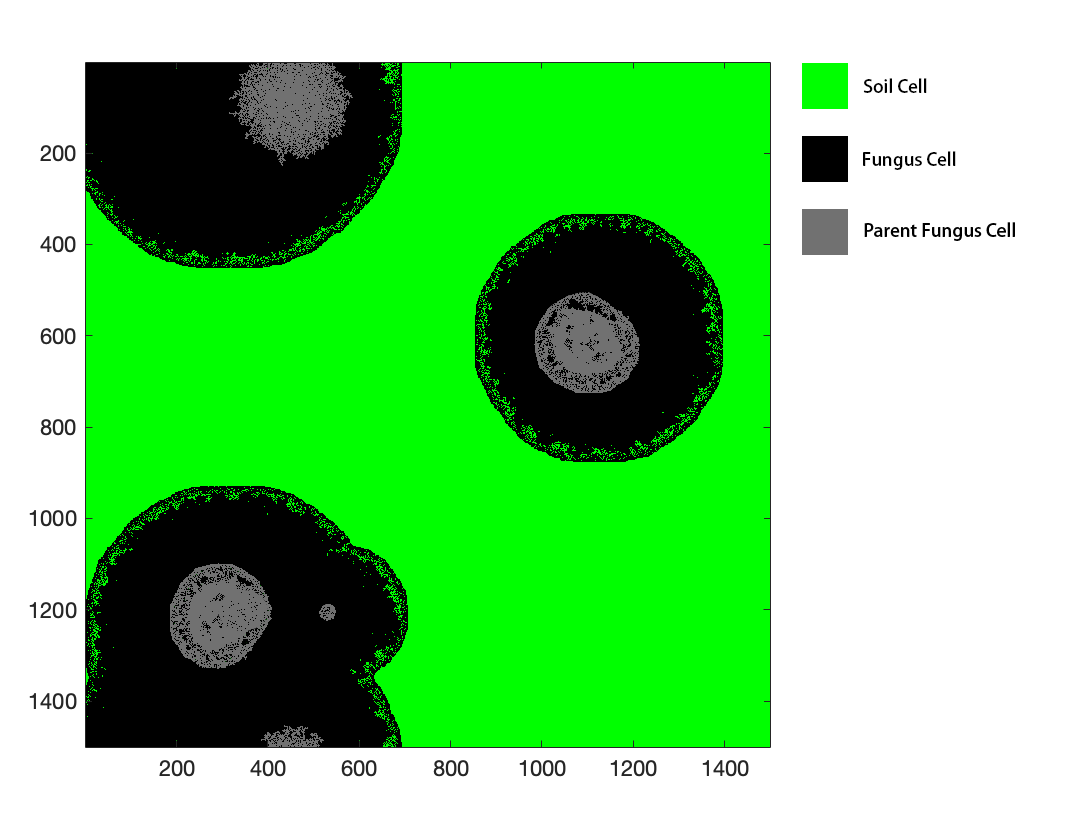
\includegraphics[width=8cm]{./pictures/cell3.png}
	\caption{SSDP at equilibrium, n=1500, Parent=5}\label{jj}
\end{figure}

\section{Sensitive Analysis}\label{condition}
The parameters are self-adjustable and has a high robustness. We use the divide-and-conquer algorithm to calculate the four direct parameters individually by WRM, then bind them up by PSM, which minimize the error when some data is missing or wrong. To prove the correctness of this analysis, we carry out the sampling experiment below.
We consider LMDP (ECMM) because this process uses most parameters and it’s our final model. The workflow is shown as below.
\begin{itemize}
\item Pick two species of parent fungus colony, align the centers of them in a rectangular form.
\item Place one center (sp. 1) inside the graph, and others (sp.2) out of the graph.
\item Give slightly different $d_S$, T, M. 
\item Run the two programs and stop them at the same time. Calculate the average growing rate of the Fungus Colony Edge of the two species, and the density of sp.1 (center of the species implying Parent Fungus Cell 1 in the graph).
\end{itemize}
The results are as follows:
\begin{figure}[H]
	\small
	\centering
	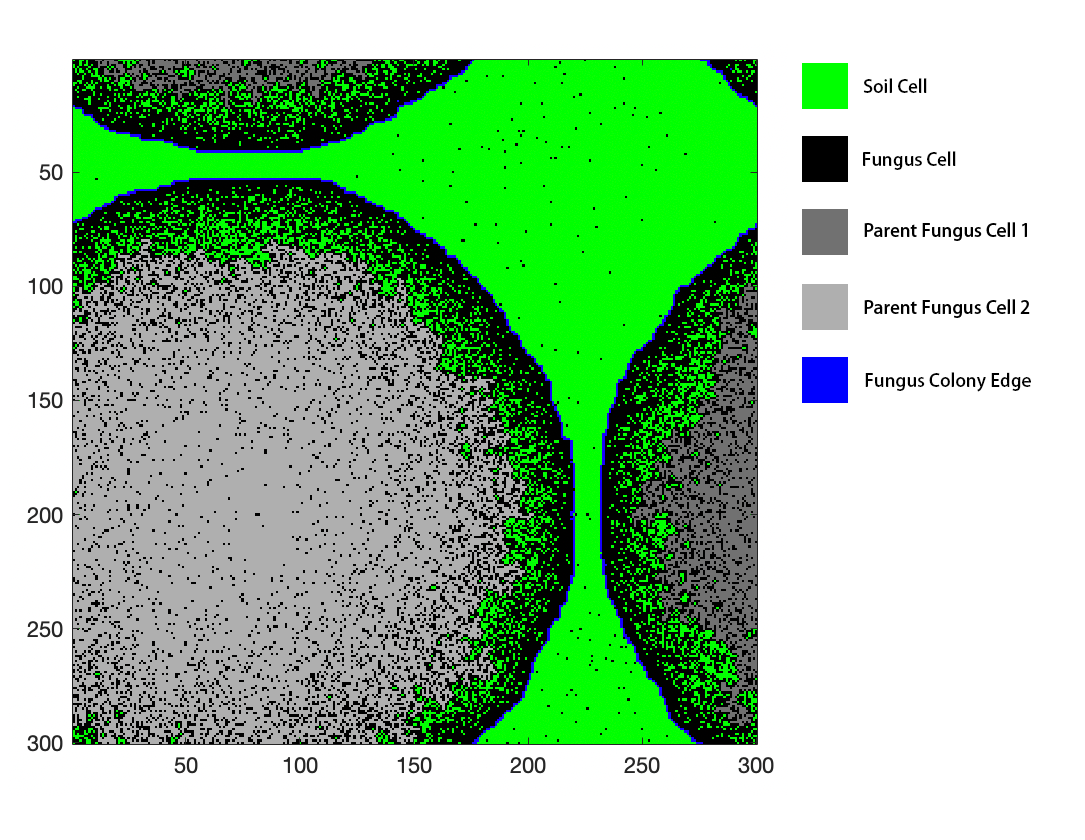
\includegraphics[width=8cm]{./pictures/1.png}
	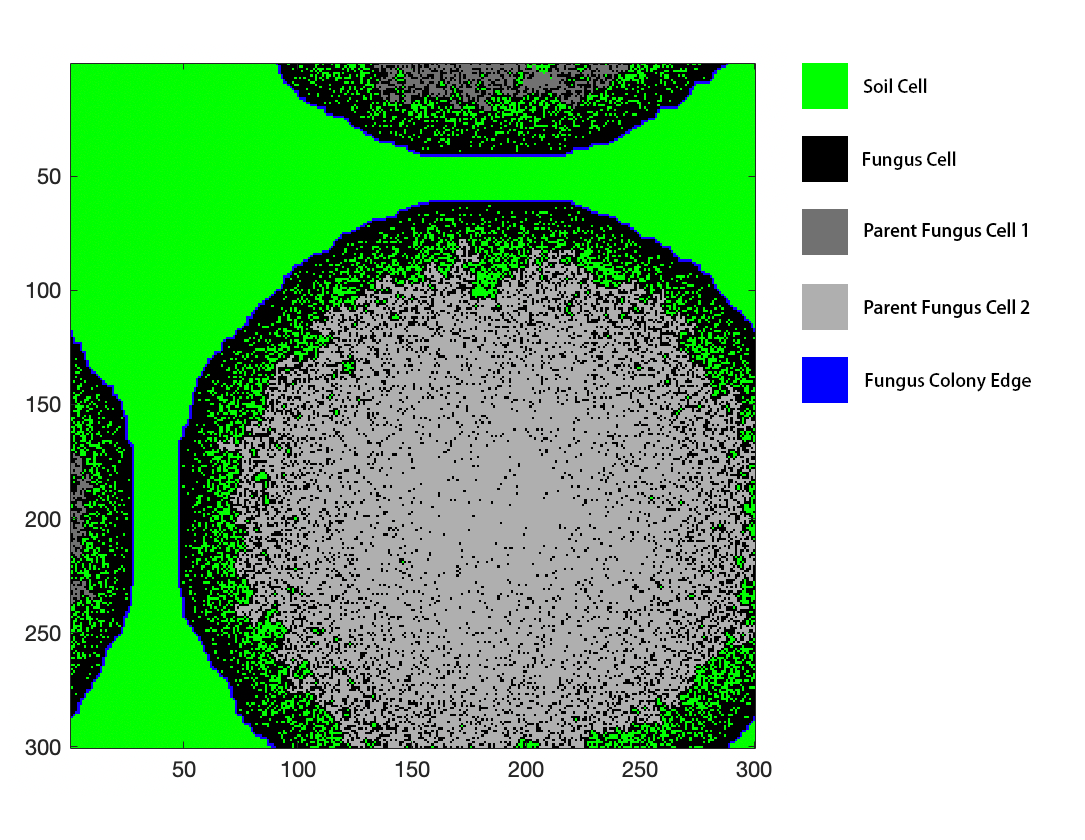
\includegraphics[width=8cm]{./pictures/2.png}
	\caption{LMDP at equilibrium, n=300, Parent=4 (left) and LMDP at equilibrium, n=300, Parent=4 (right)}\label{nt}
\end{figure}
(Notice that we choose n = 300 to gain a more intuitive sense of the fungal density. Also notice that the figure on the left has a different $d_S$ with the figure on the right.)
By calculation, we observe the system response fluctuating:

\begin{figure}[H]
	\small
	\centering
	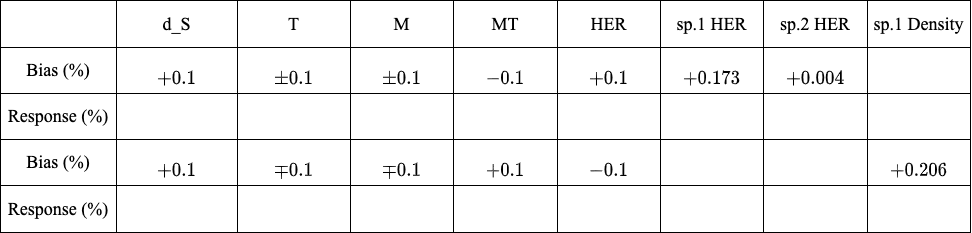
\includegraphics[width=15cm]{./pictures/t.png}
	\caption{Sensitive Analysis}\label{jj}
\end{figure}

\section{Strengths and Weaknesses}
\subsection{Strengths}
\begin{itemize}
	\item \textbf { The decomposition model describes the multi-species decomposition process and shows the contest for species to attain nutrition from environment.}
	\item The interaction model describes the competition between multiple species, and based on Markov process, computes the dominant possibility for each species. Especially, \textbf{we take the environment into the consideration to refine the original method}, and generate a approximate influence for environment to the fungi colony.
	\item \textbf{The algorithm is one-to-all.} By inputting the four indirect parameters, we’re able to select one process to gain the output graph, and we can use the model we’ve gained to examine the correctness of our conclusion, which is organized systematically.
	\item \textbf{The parameters are self-adjustable and has a high robustness.} We use the divide-and-conquer algorithm to calculate the four direct parameters individually by WRM, then bind them up by PSM, which minimize the error when some data is missing or wrong.

\end{itemize}
\subsection{Weaknesses}
\begin{itemize}
	\item The decomposition model assumes that the nutrition from environment is constantly imported from environment.
	\item One assumption is that we take “long-term” equivalent to the change of the parameters temperature and moisture, which somewhat over-simplify the question.
	\item The algorithm uses a basic method Flood Fill Recursion, which is relatively ineffective and cause the experiment process slow.
\end{itemize}
\section{Conclusion}
In conclusion, to solve the four questions asked, we’ve built two extended models and one algorithm.
\begin{itemize}
\item The first model, the Decomposition Model, is utilized to analyze the decomposition process of fungus. Firstly it’s about single-species (which cannot solve the questions asked), then we extend it to multi-species, so it can explain for the coexistence of multiple species of fungi in the decomposition process of ground litter and woody fibers. (as stated in the Problem Restatement part).
\item The second model, the Multi-species Model, is set to simulate the interactive relations between different species (based on Markov process and Patched Matrix Method) so that we can explain the expound interactions between different species of fungi including both short-term and long-term trends, and we predicted possible advantage and disadvantage for each species and combinations with variation of environmental patterns. It can also be used to describe the importance and role of biodiversity on the decomposing system and variability of environment
\item The algorithm, the High-Precision Cellular-Automaton, is set to calculate the parameters and use Flood Fill to simulate the real distribution and change of the distribution to validate the models.
\end{itemize}
\newpage



\section*{Memo}\addcontentsline{toc}{section}{Memo}

	\begin{flushleft}
		Dear users:
	\end{flushleft}
	
	Thank you very much for choosing our bathtubs. Each piece of your support is our valuable treasure
	which can encourage us to develop better bathtubs.We express our sincere thanks to you and your
	family!
	For this kind of bathtub, we have some suggestions for you:
	\begin{enumerate}[\bf 1.]
		\item You don't have to worry about the full-water condition, because when the bathtub is full
		of water, the overflow drain can drain out the excess water.
		\item With the consideration that you will have your special demands on the bath water, we give
		you some suggestion through so that you can choose what you prefer
		(or just freestyle you bath).
		
	\end{enumerate}

\clearpage
\begin{thebibliography}{99}
	\addcontentsline{toc}{section}{References}  %引用部分标题("Refenrence")的重命名
	
	\bibitem{1}Harmon, M. E., Krankina, O. N., Y atskov, M. , Matthews, E., Predicting Broad-scale Carbon Stores of Woody Detritus from Plot-level Data in Assessment Methods for Soil Carbon. \emph{CRC Press}, 2001:533-552.
	\bibitem{2}Luyssaert, S. et al, CO2 Balance of Boreal, Temperate, and Tropical Forests Derived from a Global Database. \emph{Glob. Change Biol.}, 2007(13): 2509-2537.
	\bibitem{3}Le Quéré, C. et al, The Global Carbon Budget 1959-2011. \emph{Earth Syst. Sci.}, 2013: 165-185.
	\bibitem{4}Nicky Lustenhouwer, Daniel S. Maynard, Mark A. Bradford, Daniel L. Lindner, Brad Oberle, 
	Amy E. Zanne, and Thomas W. Crowther, A Trait-based Understanding of Wood Decomposition by Fungi. \emph{PNAS}, May 13, 2020.
	\bibitem{5}Werner Ulrich et al, Matrix Models for Quantifying Competitive Intransitivity from Species Abundance Data. \emph{Nordic Society Oikos }, 2014(123): 1057-1070.
	\bibitem{6}D. S. Maynard et al, Diversity Begets Diversity in Competition for Space. \emph{Nat. Ecol. Evol.}, 2017(1): 0156.
	\bibitem{7}D. S. Maynard et al, Fungal Interactions Reduce Carbon Use Efficiency. \emph{Dryad}, June 16, 2018.
	\bibitem{8}World Meteorological Organization, Select a Monthly Time Series: Climate Indices http://climexp.knmi.nl/selectindex.cgi?id=someone@somewhere. Accessed Feb 6, 2021.
	\bibitem{9}Gilpin, M. E. Limit cycles in competition communities. \emph{Am. Nat.}, 1975(109):51-60.
\end{thebibliography}

\clearpage

\section*{Appendices}\addcontentsline{toc}{section}{Appendices}
	\subsection*{Appendix 1}
	%下面的是配置是可以写中文注释的python环境:
	%\usepackage{listings}
	%\usepackage{color}
	\definecolor{dkgreen}{rgb}{0,0.6,0}
	\definecolor{gray}{rgb}{0.5,0.5,0.5}
	\definecolor{mauve}{rgb}{0.58,0,0.82}
	\lstset{	frame=shadowbox,                           % shadowbox framed
		rulesepcolor= \color{gray},%框的颜色
		language=Python,
		aboveskip=3mm,
		belowskip=3mm,
		showstringspaces=false,
		columns=flexible,
		basicstyle={\small\ttfamily},
		numbers=left,%设置行号位置none不显示行号
		%numberstyle=\tiny\courier, %设置行号大小  
		numberstyle=\tiny\color{gray},
		keywordstyle=\color{blue},
		commentstyle=\color{dkgreen},
		stringstyle=\color{mauve},
		breaklines=true,
		breakatwhitespace=true,
		escapeinside=``,%逃逸字符(1左面的键),用于显示中文例如在代码中`中文...`
		tabsize=4,
		extendedchars=false %解决代码跨页时,章节标题,页眉等汉字不显示的问题  
	}
	\begin{lstlisting}
	from sklearn.svm import SVC
	classifier = SVC(kernel = 'rbf',C=0.8, random_state = 0,class_weight={0:20,1:24})
	#classifier = SVC(kernel = 'rbf',C=1.2, random_state = 0)
	classifier.fit(X_train, y_train)
	# Predicting the Test set results
	y_pred = classifier.predict(X_test)
	
	\end{lstlisting}
	
	

%%%%%%%%%%%%%%%%%%%%%%%%%%%%%%
\end{document}
